\chapter{ОБЗОР СУЩЕСТВУЮЩИХ РЕШЕНИЙ}\label{ch:ch1}

Разработка методов требует глубокого погружения в тематику работы, поэтому необходимо рассмотреть комплексно весь перечень проблем, встречающихся в пещерах \pic{fig:anymal_cave}. 

\begin{figure}[H]
    \centering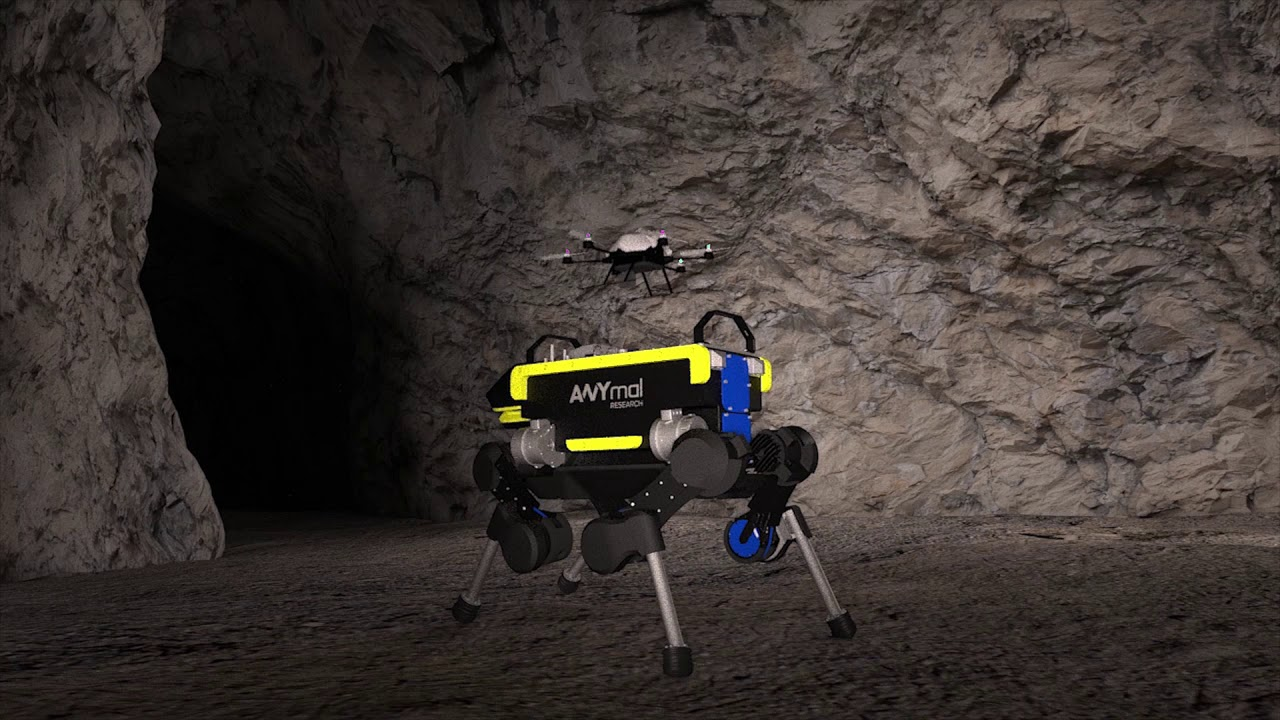
\includegraphics[height=6cm,width=1\textwidth,keepaspectratio]{anymal_cave.png}
    \caption{Пример пещеры, которую исследует робот AnyMal}
    \label{fig:anymal_cave}
\end{figure}

\section{Описание пещеры}
Пещера -- полость в верхней части земной коры, сообщающаяся с поверхностью одним или несколькими входными отверстиями. Пещеры естественного происхождения бывают следующими.
\begin{itemize}
    \item Карстовые. 
    \item Тектонические.
    \item Эрозионные.
    \item Ледниковые.
    \item Вулканические.
\end{itemize}

Начнем описание с структуры поверхностей:
\begin{itemize}
    \item твердые породы, прочные -- мрамор, кварц, базальт (магма) \pic{fig:solid_surfaces};
    \item твердые породы, мягкие -- мел, гипс, соль, известняк \pic{fig:solid_surfaces};
    \item сыпучие грунты -- песок, глина, снег \pic{fig:running_soils};
    \item водные преграды -- как и лужи (малый слой воды), так и целы залы, погруженные под воду. Часто встречаются сифоны \pic{fig:water_obstacles};
    \item скользкие поверхности -- отложения мха и плесени, лед \pic{fig:slippery_surfaces};
    \item разрушаемые поверхности -- каменная гряда, паутина.
\end{itemize}

\begin{figure}[H]
\begin{subfigure}{0.49\textwidth}
\centering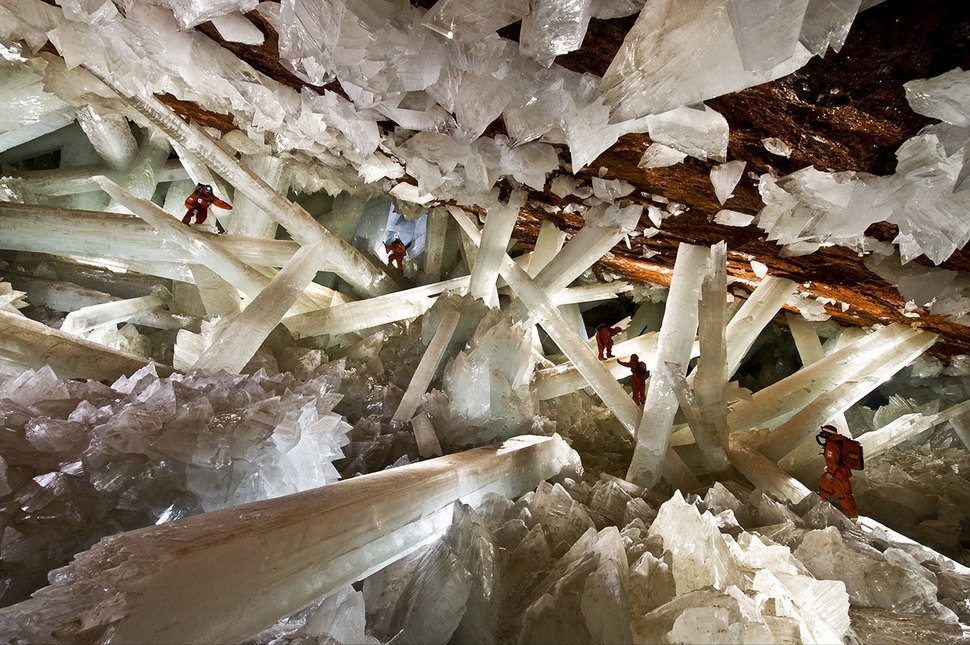
\includegraphics[width=0.99\textwidth]{surface_types/crystal.png}\\
\caption{Кристаллы}
\label{fig:crystal}
\end{subfigure}
\begin{subfigure}{0.49\textwidth}
\centering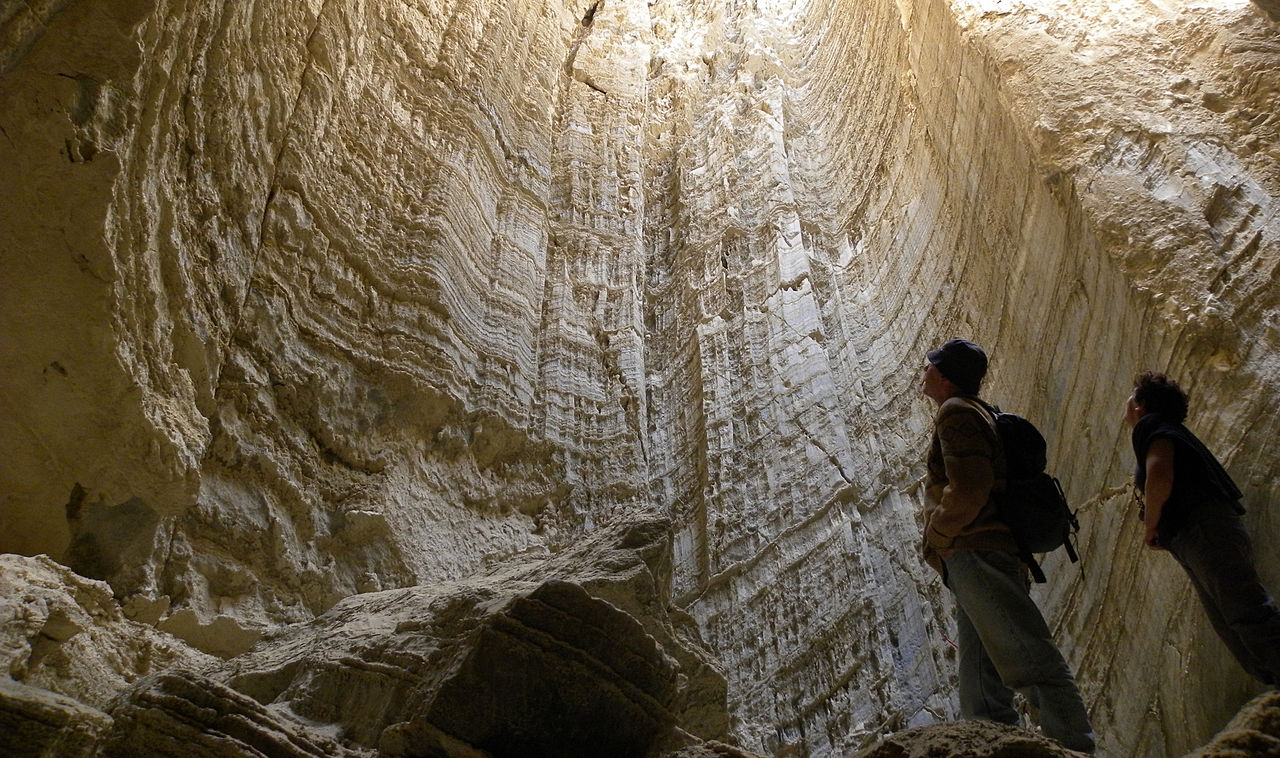
\includegraphics[width=0.99\textwidth]{surface_types/salt.jpg}\\
\caption{Солевые отложения}
\label{fig:salt}
\end{subfigure}

\begin{subfigure}{0.49\textwidth}
\centering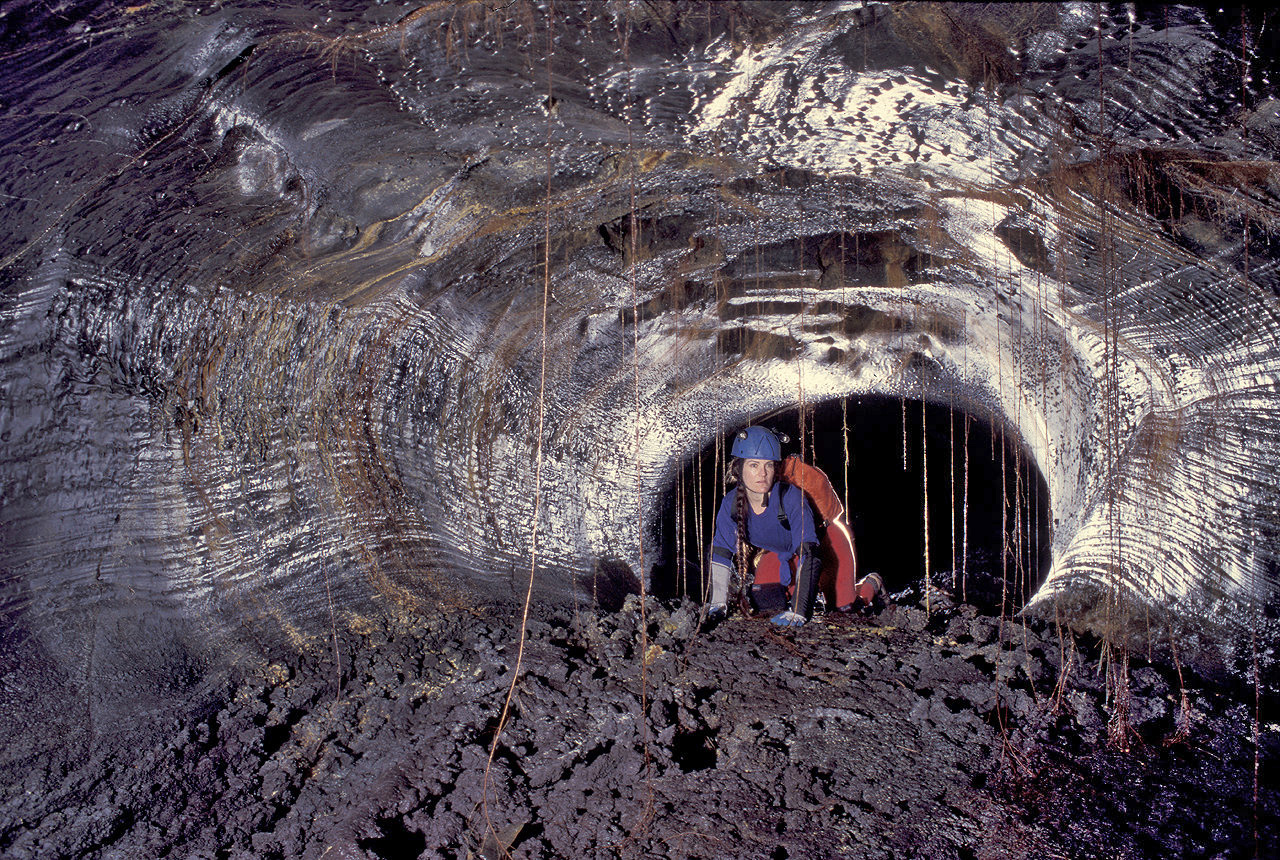
\includegraphics[width=0.99\textwidth]{surface_types/lava.jpg}\\
\caption{Магма}
\label{fig:lava}
\end{subfigure}
\begin{subfigure}{0.49\textwidth}
\centering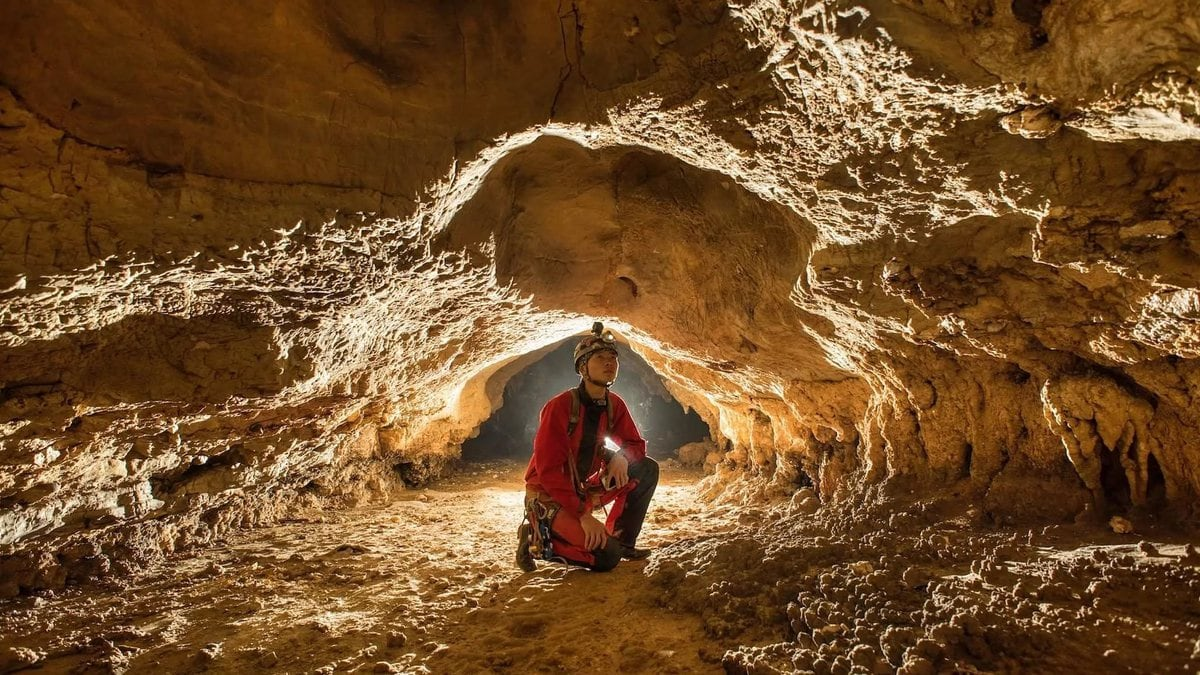
\includegraphics[width=0.99\textwidth]{surface_types/limestone.png}\\
\caption{Известняк}
\label{fig:limestone}
\end{subfigure}
\caption{Твердые поверхности}
\label{fig:solid_surfaces}
\end{figure}

\begin{figure}[H]
\begin{subfigure}{0.49\textwidth}
\centering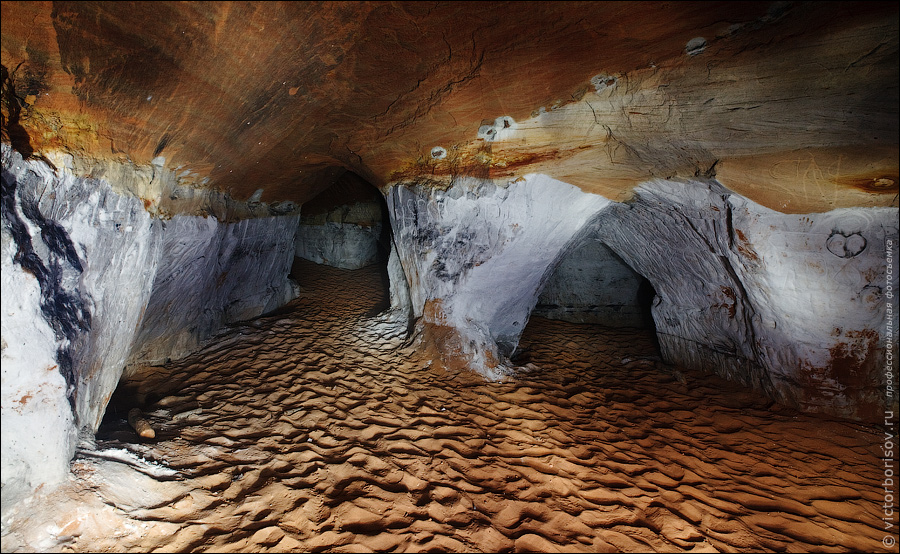
\includegraphics[width=0.99\textwidth]{surface_types/sand.jpg}\\
\caption{Песок}
\label{fig:sand}
\end{subfigure}
\begin{subfigure}{0.49\textwidth}
\centering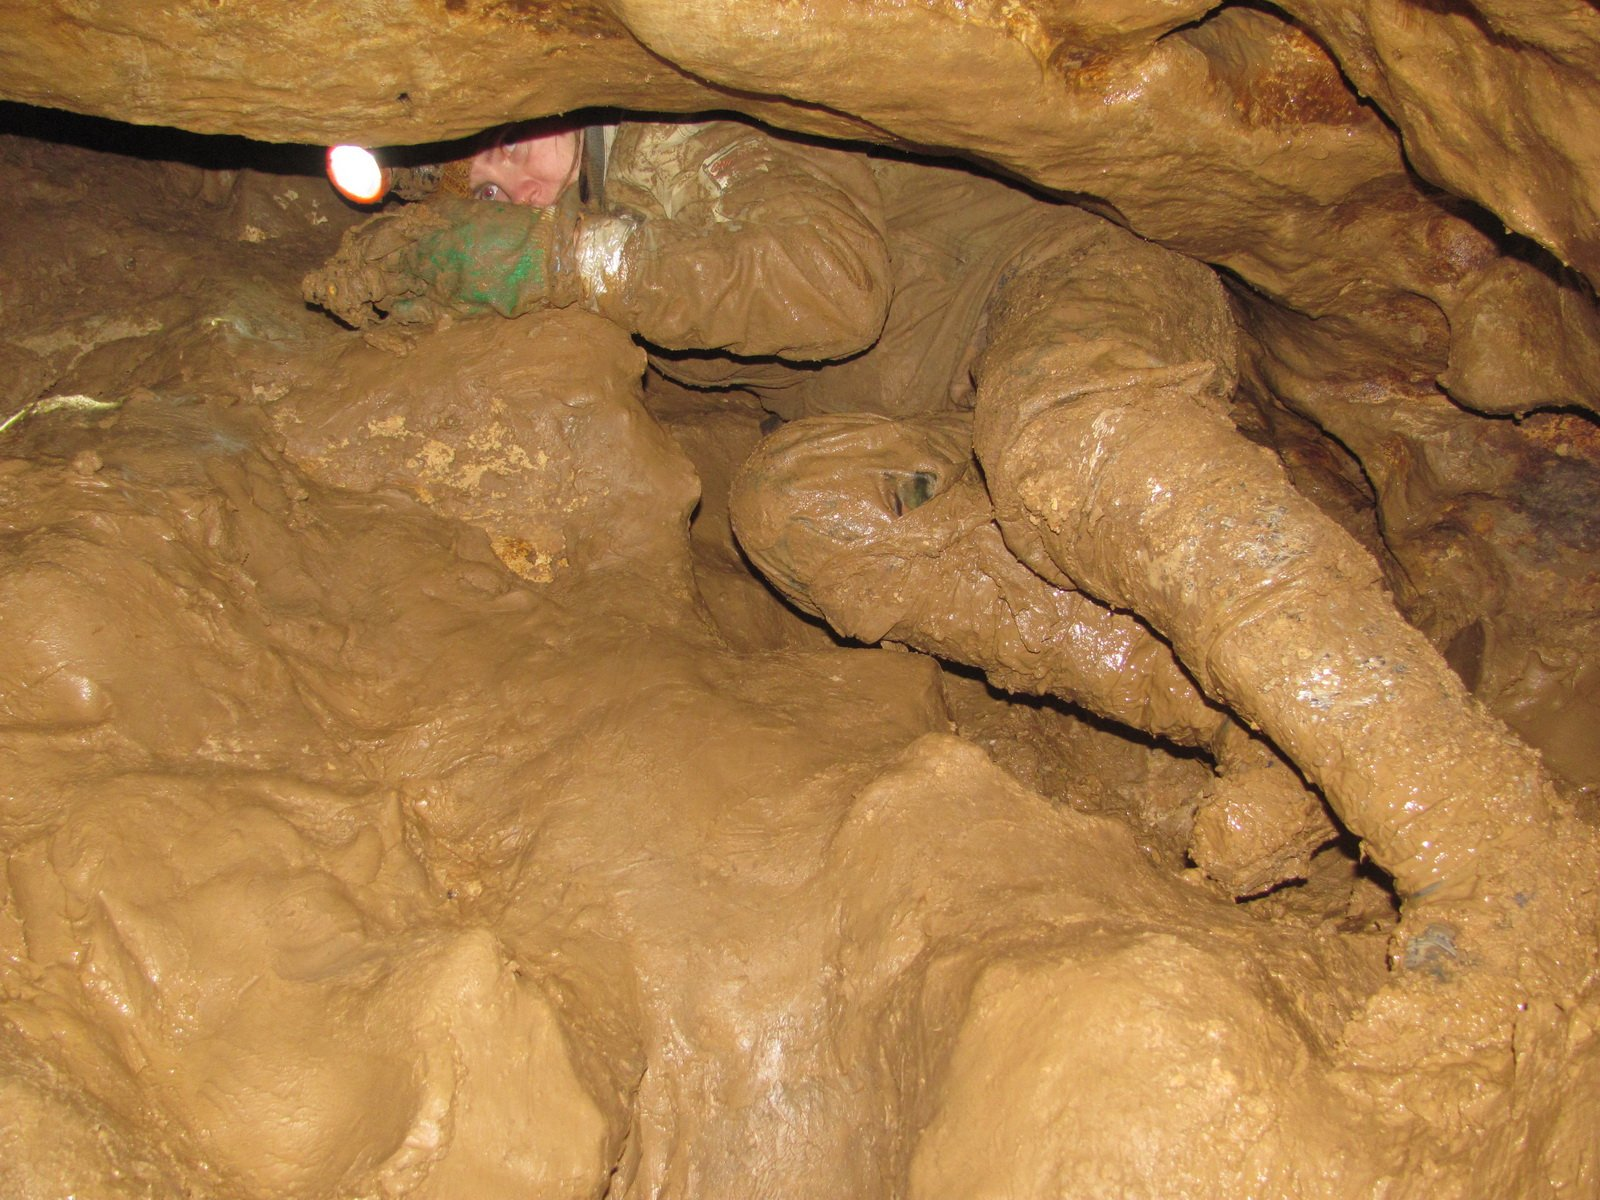
\includegraphics[width=0.99\textwidth]{surface_types/clay.jpg}\\
\caption{Глина}
\label{fig:clay}
\end{subfigure}
\caption{Сыпучие грунты}
\label{fig:running_soils}
\end{figure}

\begin{figure}[H]
\begin{subfigure}{0.49\textwidth}
\centering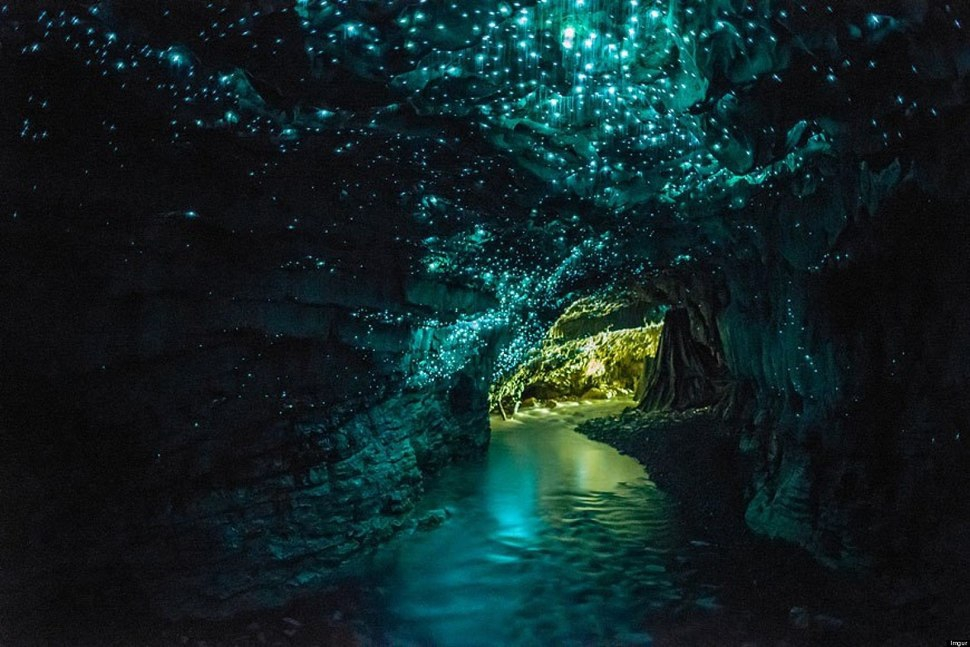
\includegraphics[width=0.99\textwidth]{surface_types/splash.png}\\
\caption{Лужа}
\label{fig:splash}
\end{subfigure}
\begin{subfigure}{0.49\textwidth}
\centering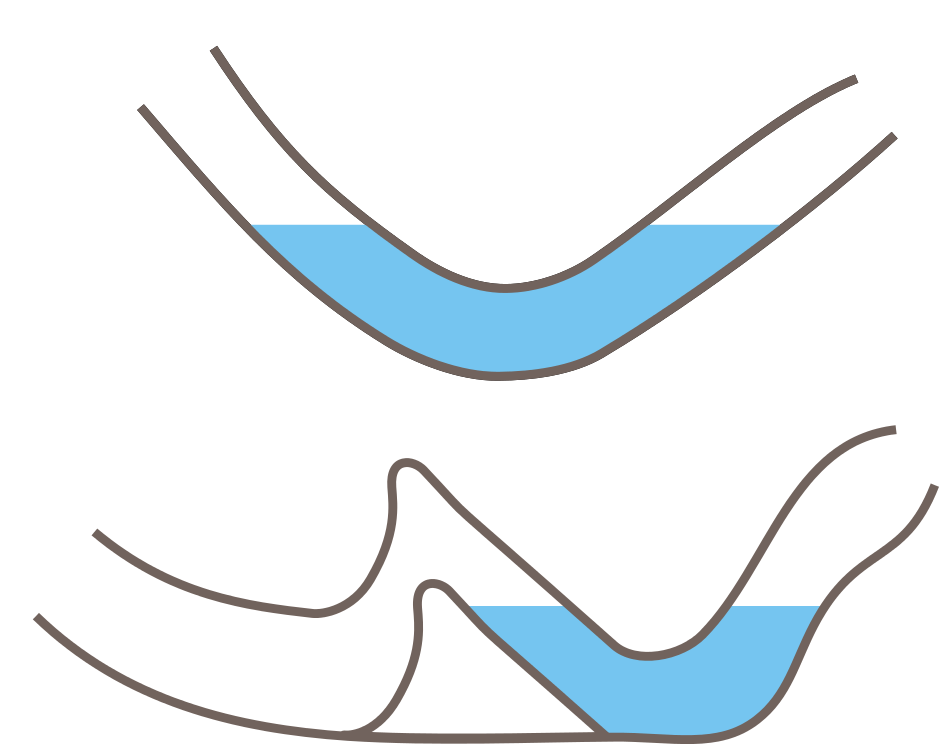
\includegraphics[width=0.99\textwidth]{surface_types/siphon.png}\\
\caption{Сифон}
\label{fig:siphon}
\end{subfigure}
\caption{Водяные препятствия}
\label{fig:water_obstacles}
\end{figure}

\begin{figure}[H]
\begin{subfigure}{0.49\textwidth}
\centering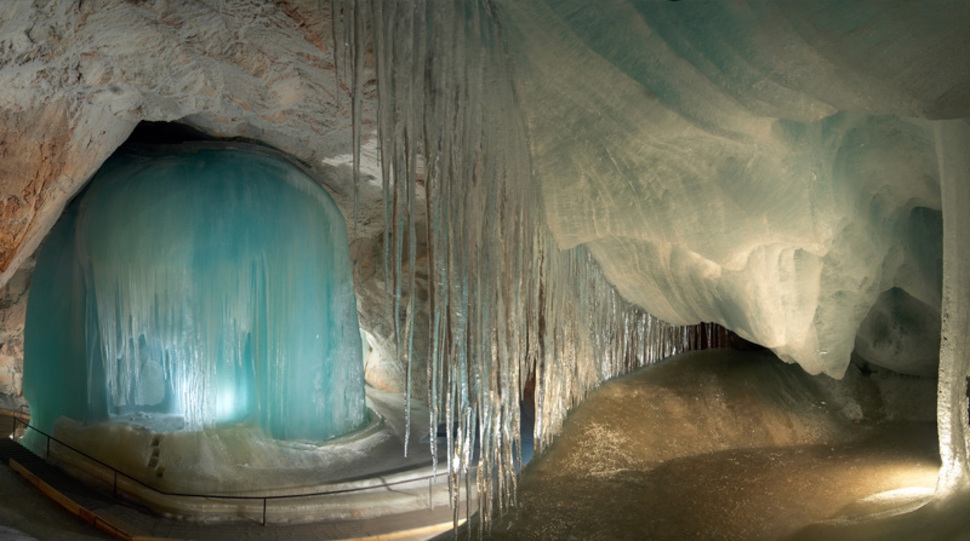
\includegraphics[width=0.99\textwidth]{surface_types/ice.png}\\
\caption{Ледяная пещера}
\label{fig:ice}
\end{subfigure}
\begin{subfigure}{0.49\textwidth}
\centering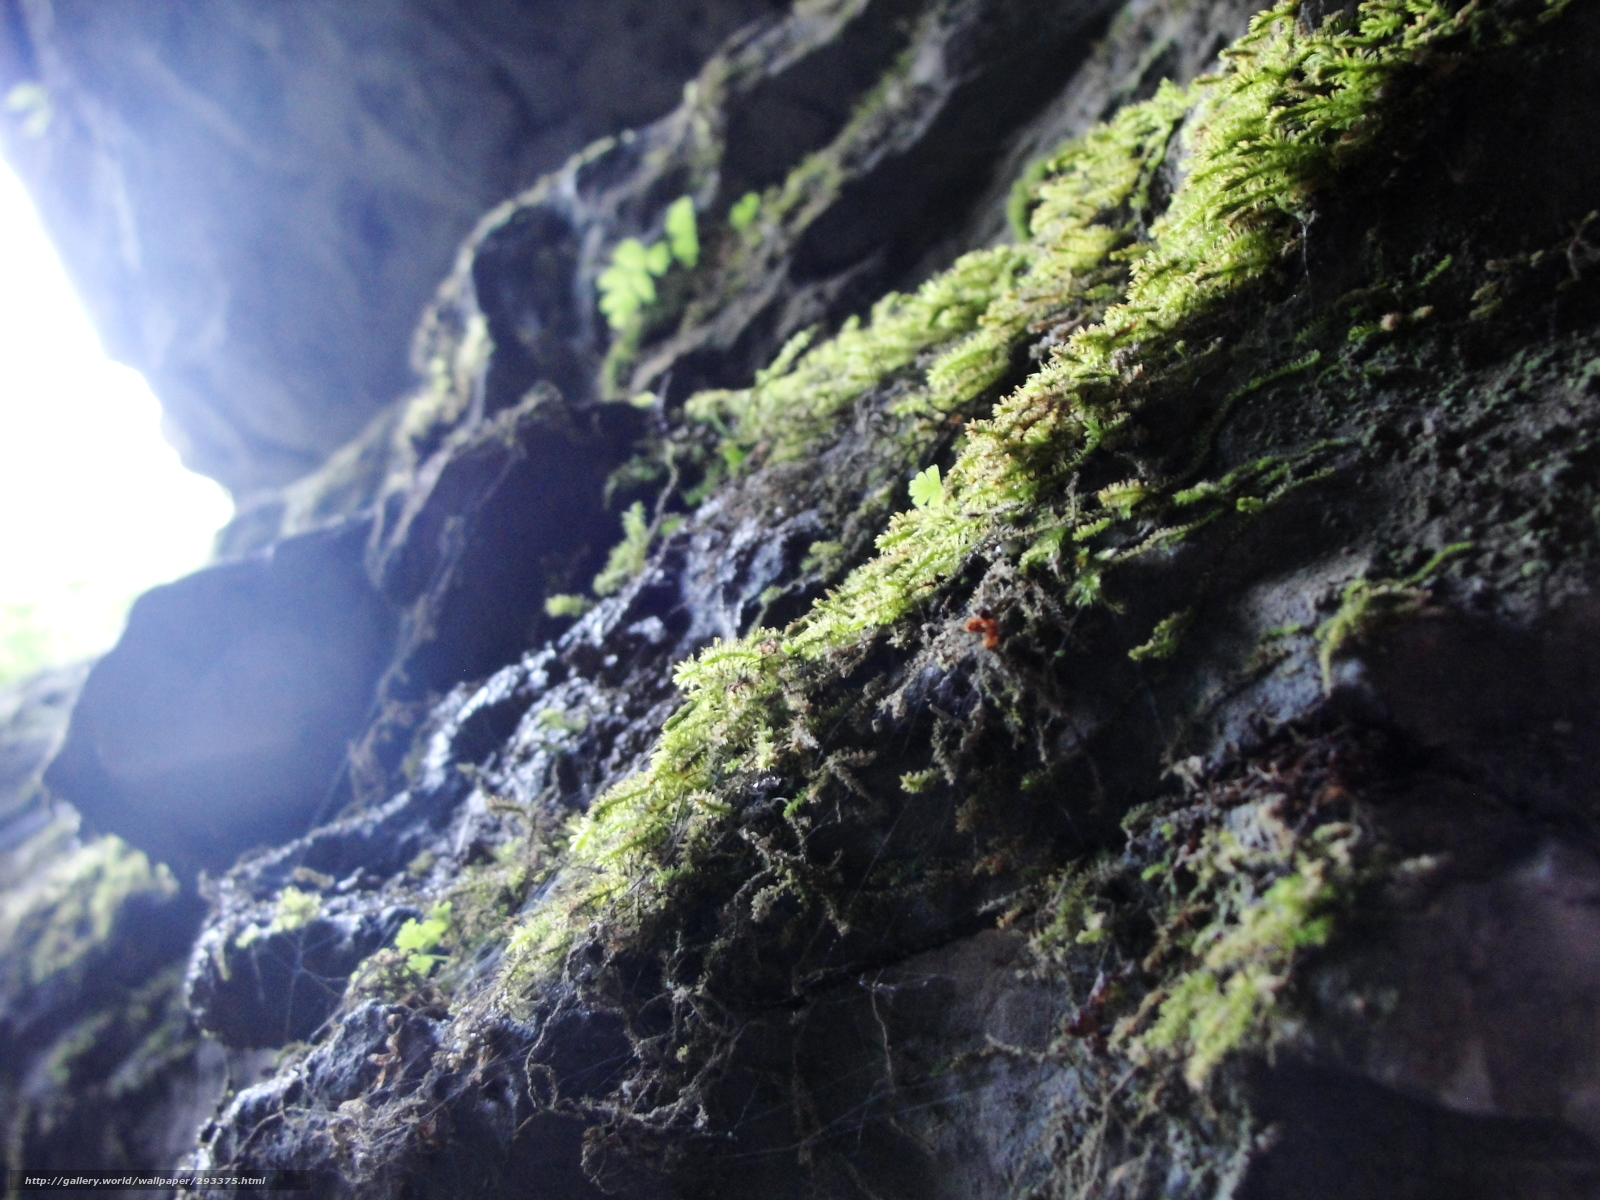
\includegraphics[width=0.99\textwidth]{surface_types/moss.jpg}\\
\caption{Мох}
\label{fig:moss}
\end{subfigure}
\caption{Скользящие поверхности}
\label{fig:slippery_surfaces}
\end{figure}

Для поставленной задачи классификация необходима, чтобы понимать какие типы препятствия и породы будут окружать робота.

Так же необходимо рассмотреть размеры пещер, чтобы понимать необходимый запас хода, размеры робототехнического комплекса. Процентное соотношение суши/воды необходимо понимать, чтобы при разработке робота понимать какой основной функционал необходим.

\begin{figure}[H]
\begin{subfigure}{0.8\textwidth}
\centering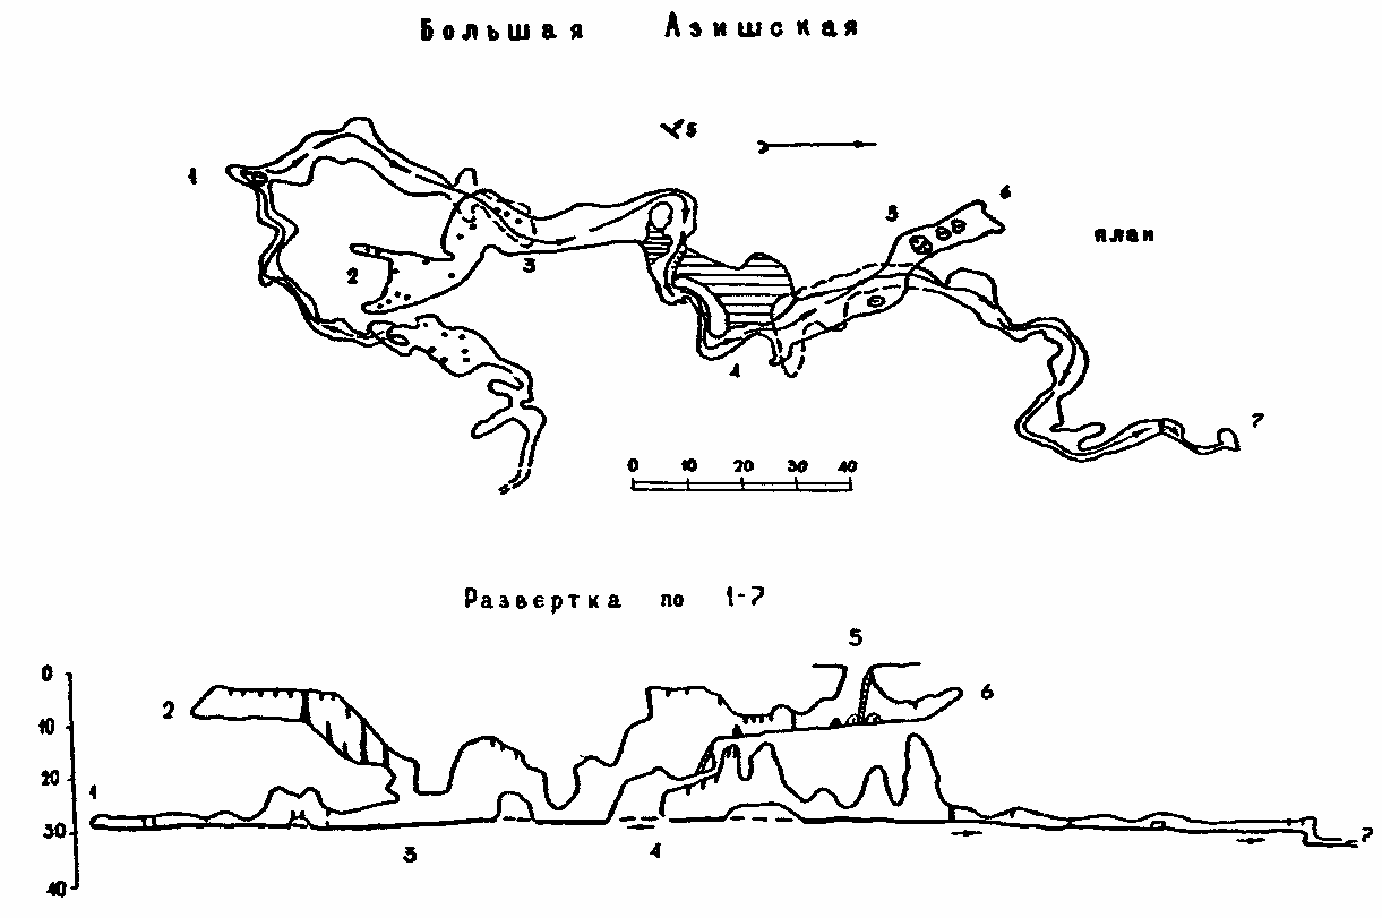
\includegraphics[width=0.8\textwidth]{cave_maps/map1.png}\\
\caption{Большая Азишская пещера}
\label{fig:ice}
\end{subfigure}
\begin{subfigure}{0.8\textwidth}
\centering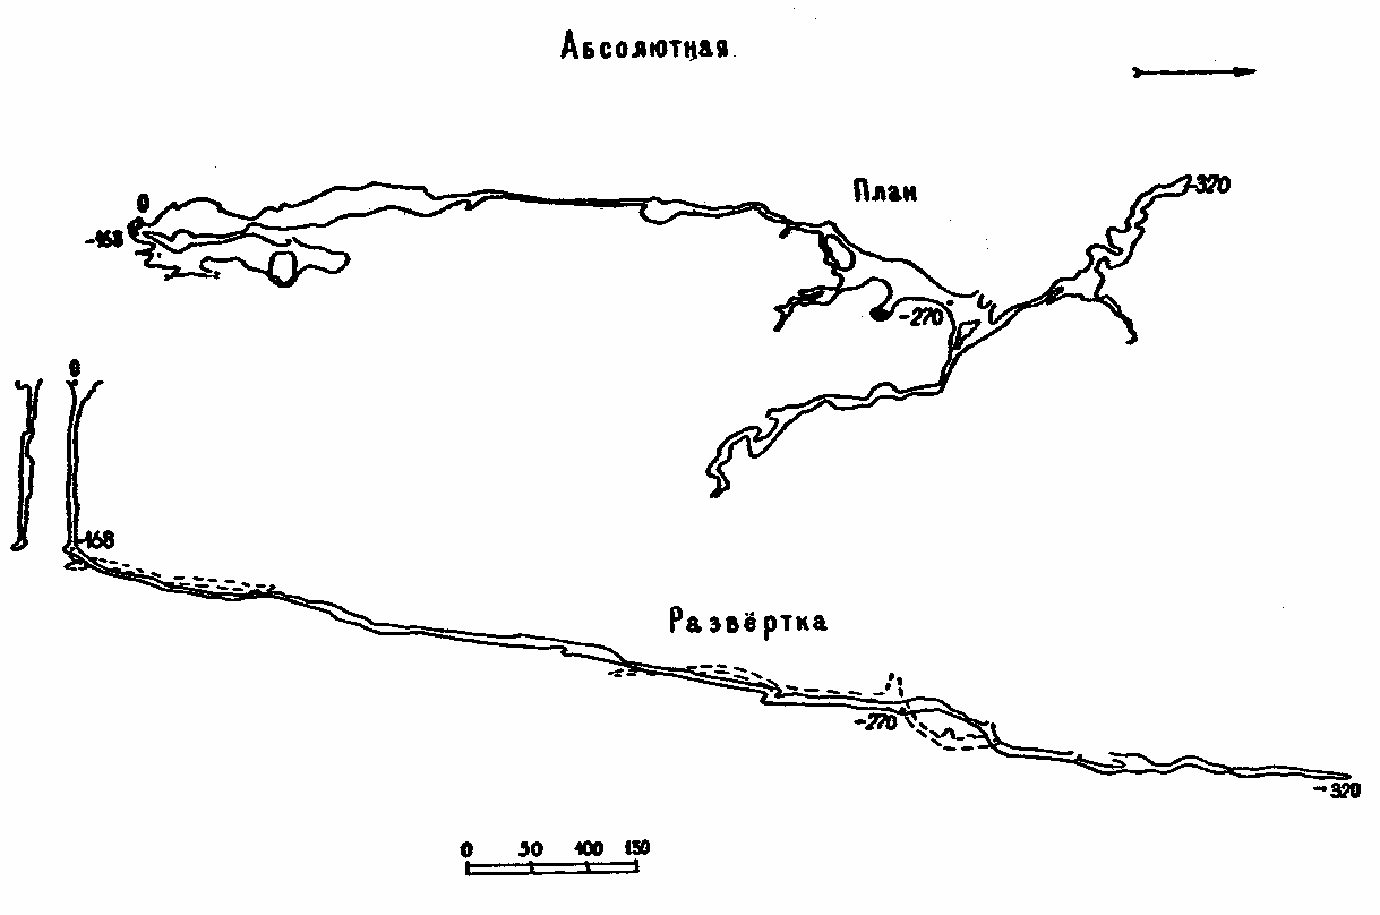
\includegraphics[width=0.8\textwidth]{cave_maps/map2.png}\\
\caption{Абсолютная пещера}
\end{subfigure}
\begin{subfigure}{0.8\textwidth}
\centering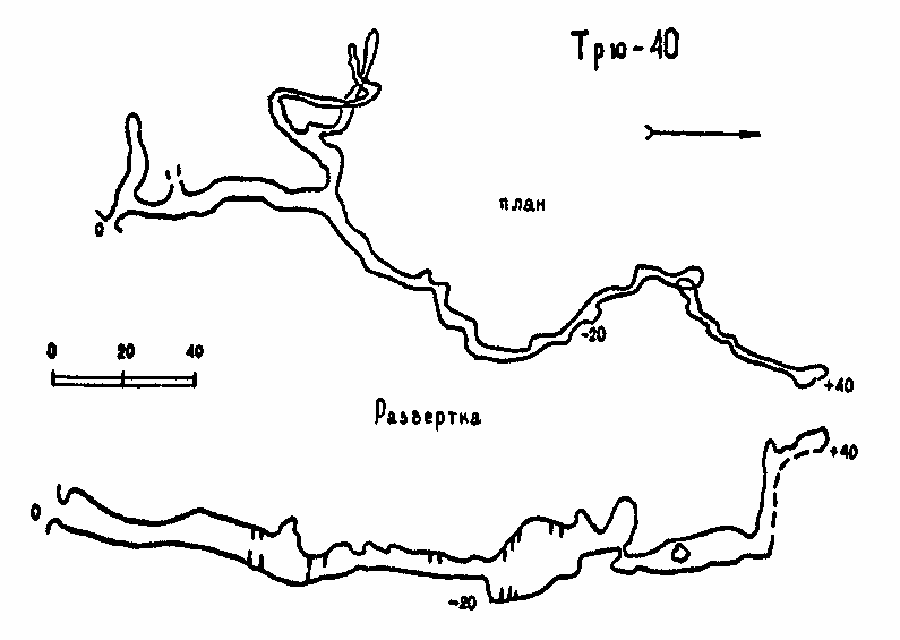
\includegraphics[width=0.8\textwidth]{cave_maps/map3.png}\\
\caption{Трю - 40}
\end{subfigure}
\caption{Размеры пещер}
\end{figure}

Основная проблема, что существуют карты тех пещер, в которые человек может пройти. Но карты пещер, куда человек не может попасть из-за своих размеров -- отсутствуют. Поэтому определение необходимых размеров остается важной задачей.

\section{Роботы, которые могут использоваться для исследования пещер}

Исследование пещер естественного происхождения является комплексной задачей, сопряженная со множественными трудностями \cite{Zhang2017a, Frumkin2019}. Деградация сенсоров \cite{Huang2019}, перебои в коммуникации между роботами из-за потери сигналов \cite{Vaquero2018, Thangavelautham2017}, сложный рельеф пещер \cite{Thangavelautham2017}, обилие грязи \cite{Baker2004}, жидких препятствий \cite{Morris2006}, требующие герметизацию корпуса, являются только малой частью встречаемых проблем в пещерах. 

Для исследования пещер роботами необходимо вначале понять, что такое пещера, какие типы существуют и какие проблемы они несут. Для робототехников важно понимать типы препятствий (от этого зависит тип движителя робота), влияние окружения на алгоритмы навигации. В пещерах возможно встретить почти все типы поверхностей, с которыми приходится сталкиваться роботам в мире. Это и твердые поверхности: мрамор, кварц, базальт. Сыпучие грунты, такие как: мел, гипс, соль, известняк. Часто встречаются водные препятствия — как лужи, так и целы залы, погруженные в воду. Особую опасность для человека вносят сифоны. Это пещера в виде параболы, где в локальном минимуме все затоплено. Скользкие поверхности: лед, мох, глина, а так же разрушаемые поверхности — каменная гряда и паутина \cite{1960,1963,1969,1971}. Все это вносит свои коррективы на выбор сенсоров. Так же важно понимать габариты пещер. Это влияет на необходимую автономность робототехнической системы \cite{Mascarich2018a}. 

Для преодоления сложного рельефа исследователи со всего мира предлагали различных роботов, робототехнические системы и типы движителей \cite{Morris2006a}. Имеет смысл рассматривать, как возможных, так и реально применяющихся для исследования пещер. Разрушение пещер нежелательно, поэтому роботы, которые для перемещения ломают породу не будут рассматриваться \cite{Semini2016}. В пещерах принято использовать, как наземных роботов, так и летающие аппараты, так и их комплексы. Из летающего транспорта это коптеры \cite{Papachristos2019,Scaramuzza2014,Zingg2010} и дирижабли \cite{Huang2019}. Дирижабль намного более автономен и может нести большую нагрузку. Наземных роботов очень много типов, но основными являются: шагающие \cite{Tan2016,Lynch2019} колесные \cite{Molyneaux2016,Vaquero2018}, трековые \cite{Reddy2015} и необычные. Необычные это роботы, которые не поддаются классификации, например змеевидные \cite{Ye2007,Borenstein2007}, шарообразные \cite{Thangavelautham2017,Dubowsky2008,Dang2019} и другие.

Но самыми эффективными являются не одинокие роботы, но системы. В данных системах появляются дополнительные задачи, как архитектурного характера, телекоммуникационного и управленческого. Обычно системы состоят из нескольких одинаковых роботов \cite{Vaquero2018}, либо связка – коптер и шагающий \cite{Chen2010,Cantelli2013}.

Отдельным пластом роботов являются ползающие роботы \cite{Schmidt2013}, которые рассматриваются автором как перспективные в пещерах. К сожалению, пещерные роботы были найдены только для космических пещер \cite{Parness2017}. Крепления для шагающих роботов устанавливают во всевозможных роботов, от шагающих и колесных, до специально разработанных под ползанье. Важным критерием для успешного робота, который может перемещаться по вертикальным поверхностям является способ адгезии с поверхностью. Существуют магнитный \cite{Lee2012,Tavakoli2012,Kotay1996,Xu2017}, электрический \cite{Li2017}[33], негативного давления \cite{Lee2012,Tavakoli2012,Papachristos2019}, пневматический или помощью присосок \cite{Nagakubo1994,Tlale2012}, и с помощью когтей (механическая адгезия) \cite{Parness2017,Bretl2006,SangbaeKim2005,Sintov2011}. Последний способ является самым применимым для пещер, так как стены очень рельефные.

Навигация в пещерах является нетривиальной задачей, поэтому необходимо рассмотреть какие сенсоры и алгоритмы, а также архитектурные решения использовались для преодоления проблем. Представленные статьи были взяты не только из прямой сферы, но также из смежных. К примеру, исследование трубопровода \cite{Savin2017}, завалов после техногенных катастроф. С точки зрения навигации основной проблемой является недостаток света, а также сильной неоднородности территории и обилия гранулированных поверхностей. На данный момент ученые мира стали стремиться решить данную проблему, благодаря проходящему соревнованию DARPA Subterranean Challenge. В данном направлении используются как лазерные дальномеры (лидары), так и визуальные SLAM алгоритмы \cite{Mascarich2018a,Dang2019a,Fairfield2006,Chhaniyara2012}. С точки зрения архитектуры, наблюдается тенденция к модульности, а также к возможным защитам от потерь робота \cite{Miller2019,Wei2009}. То есть, если робот был потерян, то остальные роботы все равно должны передавать друг другу данные. Очень важно уметь правильно передвигать робота по сыпучим грунтам, следующие работы посвящены этим проблемам. Основной критерий это решение задачи в настоящем времени \cite{Tan2016,Savin2017,Chhaniyara2012,Tsounis2019, Li2009,Bjelonic2019,DeViragh2019,Buchanan2019}.

Целью данной аспирантской работы является разработка метода, который поможет получить информацию по поверхности пещеры. Обычно под этим подразумевается только получения типа поверхности, эти статьи и были рассмотрены \cite{Wu2016,Wu2020,Luo2017}.

Подведя итог, в данном обзоре были представлены причины проблем, возникающие при разведке пещер роботами. Были описаны типы пещер, рассмотрены их размеры. Представлены варианты возможных препятствий, а также сделаны выводы как это влияет на робототехническую систему. После этого показаны решения, предложенные исследователями по всему миру, связанные с навигацией, подбором движителя, выбором сенсоров и архитектурными решениями, дающие надежную систему. 

Ходьба, прыжки, скачки, бег и ползание предполагают что связи ног с опорной поверхностью является неудерживающими. Однако ноги могут быть снабжены специальными устройствами — захватами, присосками и.т.п., позволяющими аппарату реализовывать удерживающие связи с опорной поверхностью. Тип движения такого аппарата называется \textit{лазанием}.

Данная классификация основана на  \cite{Maloletov2015dinamica} работе. С помощью ног могут реализовываться локомоции различных типов. \textit{Ходьбой} называется такой тип движения машины, при котором в каждый момент времени хотя бы один механизм шагания находится в опоре. Если фаза движения машины с опорой на ноги перемежается фазой покоя, в которой машина неподвижно лежит на опорной поверхности, то такое движение называется \textit{ползанием}. Если существуют такие моменты времени когда ни одна из ног машины не контактирует с опорой, то такие движения называются \textit{прыжками, скачками или бегом}.

\subsection{Классификация шагающих машин}

На основе данной классификации, разрабатываемый робот входит в состав группы ''Шагающие циклового действия''.

\subsection{Типы мобильных робототехнических комплексов}
Для работы на земле была разработана концепция \textit{Мобильного Робототехнического Комплекса} (МРК) -  совокупность программно-алгоритмических и аппаратных решений обеспечивающих комплексную автоматизацию выполнения группы поставленных задач. Предназначен для ведения войсковой разведки, огневой поддержки войсковых подразделений, охраны и обороны военных объектов, мест дислокации, установки датчиков КРСС различного типа.
\section{Обзор существующих мобильных робототехнических комплексов}
Мобильные робототехнические комплексы применяются при:
\begin{itemize}
\item боевом обеспечении спецопераций (заградительный огонь, разведка боем, разрушение заграждений и т. п.);
\item проведении разведки;
\item проведении взрывотехнических работ (поиск, извлечение, транспортирование и обезвреживание или уничтожение взрывоопасных предметов и неразорвавшихся боеприпасов; взрывные работы);
\item обеспечении безопасности важных объектов.
\end{itemize}

По массе и основному назначению МРК можно разделить на четыре группы \tab{tab:mrk_types}:
\begin{itemize}
\item сверхлегкие, массой до 35 кг;
\item легкие, массой до 150 кг;
\item средние, массой до 800 кг;
\item тяжелые, массой свыше 800 кг.
\end{itemize}

Разрабатываемый робот принадлежит к сверхлегким роботам. Это объясняется постановкой задачи. Так как роботу необходимо преодолевать сложные узкие препятствия.
\begin{small}
\begin{center}
\begin{longtable}[H]{|p{2cm}|p{3cm}|p{3cm}|p{3.2cm}|p{3cm}|}
%Костылина для таблиц, чтобы по ГОСТу было название
\caption{Классификация МРК }\\
\label{tab:mrk_types}
% \multicolumn{5}{l}%
% {\normalsize{Таблица \thetable ~--- Классификация МРК} \label{tab:mrk_types}}\\
% \hline
\normalsize{Группа} & \normalsize{Назначение} & \normalsize{Мобильность} & \normalsize{Особенности конструкции} & \normalsize{Оснащение}\\
\hline
\endfirsthead
\multicolumn{5}{l}%
{\textit{\normalsize{Продолжение таблицы \thetable}}}\\
\hline
\normalsize{Группа} & \normalsize{Назначение} & \normalsize{Мобильность} & \normalsize{Особенности конструкции} & \normalsize{Оснащение}\\
\hline
\endhead
\hline
\endlastfoot
\normalsize{Сверх\-легкие} 
&
Визуальная и акустическая разведка в помещениях и в объектах транспорта. Осмотр труднодоступных мест (днища автомобилей и т.п.) и разрушение обнаруженных СВУ.
&
Перевозка любым видом транспорта в контейнере-чемодане. Выгрузка оператором. Переноска оператором или доставка с помощью более тяжелых МРК к исследуемому объекту. 
&
Шасси гусеничное, колесное или специальное комбинированное. Управление по радио, волоконно-оптической линии связи (ВОЛС) или кабелю. Питание от аккумуляторов. 
&
1-4 малогабаритных черно-белых или цветных камеры 
1-2 гидроразрушителя. \\ 
\hline 
\normalsize{Легкие}
&
Разведка внутри помещений и на открытой местности. Проведение взрывотехнических работ.
&
Перевозка легковым автомобилем с кузовом <<универсал>>. Выгрузка вручную (2-4 чел.) или своим ходом по аппарелям. Возможна переноска на относительно небольшие расстояния.
&
Шасси гусеничное, колесное или специальное комбинированное. Управление по радио, ВОЛС или кабелю. Питание от встроенных аккумуляторов или от сети по кабелю до 100 м.
&
1-4 телекамеры. Стрела кранового или телескопического типа, либо манипулятор с 2-5 степенями подвижности. самозарядное ружье. комплекты взрывотехнического и разведывательного оборудования. \\ 
\hline 
\normalsize{Средние} 
&
Разведка, наблюдение, охрана, проведение взрывотехнических работ. Носитель легкого стрелкового и ракетного вооружения.
&
Перевозка микроавтобусом или легким грузовиком. выгрузка своим ходом по аппарелям.
&
Шасси гусеничное, колесное или специальное комбинированное. Управление по радио, ВОЛС или кабелю. Питание от встроенных аккумуляторов 
&
2-4 телекамеры. Манипулятор с 2-6 степенями подвижности и сменным инструментом. Самозарядное ружье, пулемет, гранатомет, ракетная пусковая установка. \\ 
\hline 
\normalsize{Тяжелые}
&
Разведка, наблюдение, патрулирование, проведения взрывотехнических работ. Носитель легкого пушечного и тяжелого стрелкового вооружения
&
Перевозка на большие расстояния специальным автотранспортом или в стандартных транспортных контейнерах. Выгрузка своим ходом или с помощью крана.
&
Шасси гусеничное, колесное или специальное комбинированное. Возможно использование серийно выпускаемых транспортных средств. Управление по радио, ВОЛС или кабелю;  
&
3-4 камеры. Манипулятор с 4-6 степенями подвижности и сменным инструментом. Пулемет, малокалиберная автоматическая пушка. Комплекты взрывотехнического и разведывательного оборудования. \\  
\hline 
\end{longtable}
\end{center}
\end{small}


\subsection{Исследования с похожими роботами}
Похожие роботы, такие как Boston Dynamics RHex \cite{altendorfer2001rhex}, Gakken Mechamo Centipede \cite{miller2008extreme}, Quattroped and TurboQuad \cite{chen2014quattroped,chen2017turboquad}, а так же Whegs \cite{schroer2004comparing} были рассмотрены. На основе данных было решено, что робот должен быть в длину меньше метра, в ширину --- меньше 70 см (стандартная ширина дверного проема). Иметь меньше 32 лапок и высота лапки должна быть больше 10 см.

В последней итерации робота получилось 1м 2 см, ширина -- 50 см, а высота лапки --- 180 мм. Длина робота очень сильно зависит от длины лапки в данных типах движителей.

\begin{figure}[H]
    \centering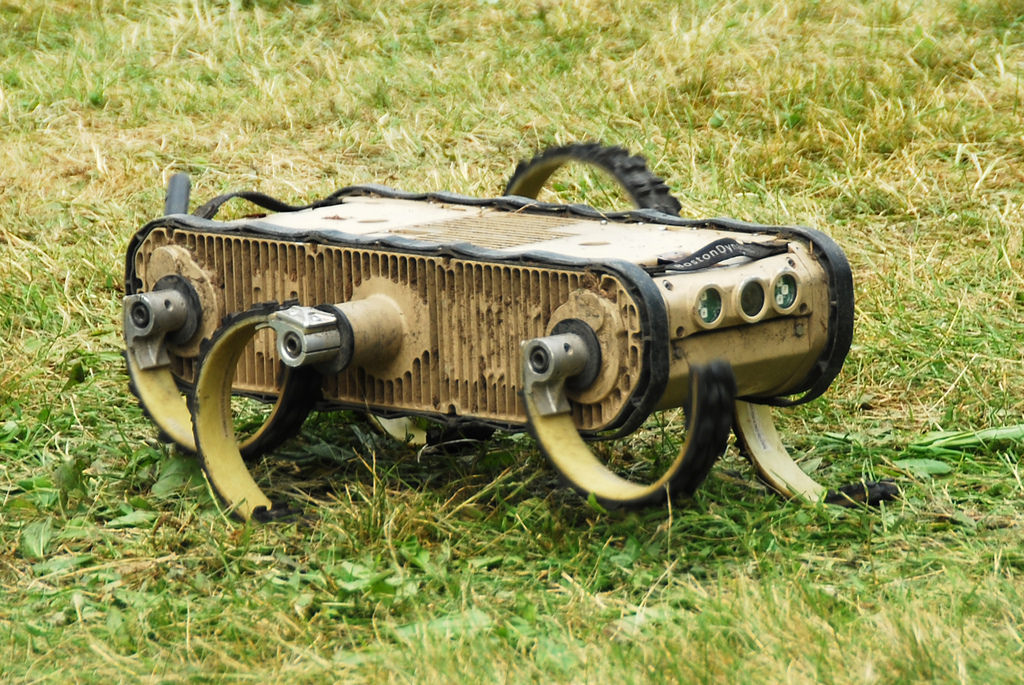
\includegraphics[width=0.6\textwidth]{from_master/rhex}\\
    \caption{Boston Dynamics робот RHex}
    \label{fig:rhex}
    \end{figure}

    \begin{figure}[H]
        \centering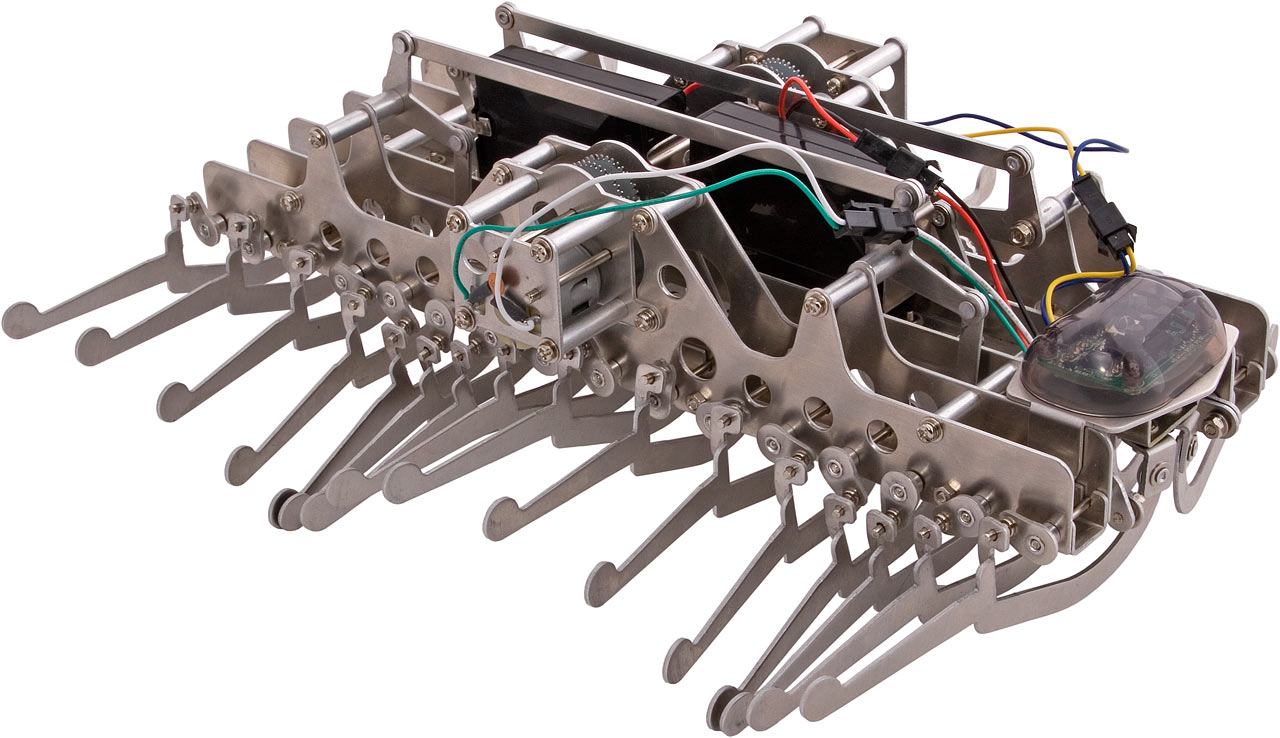
\includegraphics[width=0.6\textwidth]{from_master/gakken}\\
    \caption{Gakken Mechamo Centipede робот}
    \label{fig:gakken}
    \end{figure}

    
    \begin{figure}[H]
    \begin{subfigure}{0.49\textwidth}
    \centering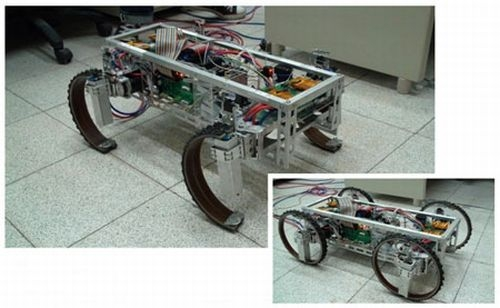
\includegraphics[width=0.9\textwidth]{from_master/quattroped}\\
    \caption{Quattroped robot}
    \label{fig:quattroped}
    \end{subfigure}
    \begin{subfigure}{0.49\textwidth}
    \centering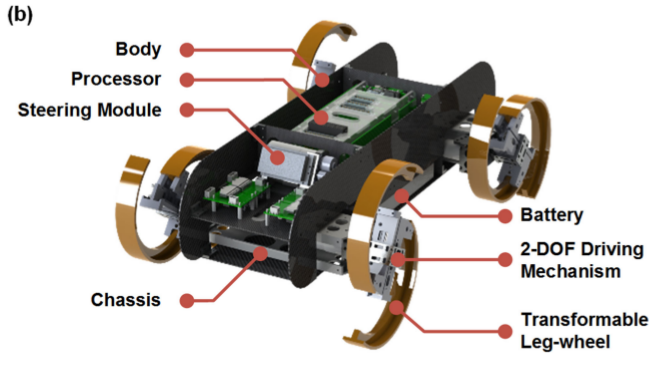
\includegraphics[width=0.9\textwidth]{from_master/turboquad}\\
    \caption{TurboQuad robot}
    \label{fig:turboquad}
    \end{subfigure}
    \caption{Quattroped семья роботов}
    \label{quatro}
    \end{figure}
    
    \begin{figure}[H]
    \centering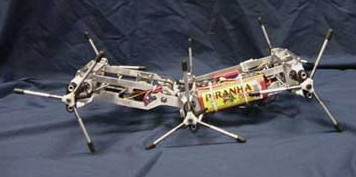
\includegraphics[width=0.7\textwidth]{from_master/whegs2}\\
    \caption{Whegs II робот}
    \label{fig:whegs}
    \end{figure}

\section{Классификация сенсорных устройств}
Информация, поступающая с различных сенсорных устройств, используется в системе управления робота для обнаружения и распознавания объектов внешней среды, построения цифровой модели, а также для управления движением робота и его манипуляторов при выполнении различных технологических операций. В соответствии с этим указанные выше две группы сенсорных устройств можно ' описать иначе следующим образом: для выявления свойств внешней среды, отдельных объектов и обеспечения перемещения исполнительных органов.

К первой из указанных групп относятся сенсорные устройства, предназначенные для выявления различных физико-химических .свойств объектов среды, включая в частности устройства для выявления параметров рельефа в рабочей зоне подвижных роботов, специальных признаков для обнаружения и распознавания определенных объектов, положения и их ориентации в рабочей зоне относительно робота и т. п.

Ко второй группе относятся датчики обратной связи (положения, скорости, ускорения), усилий, возникающих при взаимодействии робота с внешней средой, прикосновения, проскальзывания и т. д.

Такое разделение сенсорных устройств достаточно условно, поскольку, например, сенсорные устройства первой группы могут быть использованы и для определения положения захвата манипулятора робота в рабочей зоне, т. е. играть роль датчиков обратной связи при управлении движением.

Сенсорные устройства робота могут воспринимать информацию на различных расстояниях от ее источника. По этому признаку сенсорные устройства делятся на сверх ближние, ближние, дальние и сверхдальние (работающие вне рабочей зоны).

Сенсорные устройства сверх ближнего действия используют для очувствления захватов и других частей манипуляторов, а также корпуса робота. Они позволяют фиксировать их контакт с объектами внешней среды (тактильные датчики), измерять усилия, возникающие в месте взаимодействия (силометрические датчики), фиксировать проскальзывание объектов.

Сенсорные устройства ближнего действия обеспечивают получение необходимой информации в непосредственной близости от робота, но бесконтактным способом. К таким устройствам относятся локационные сенсоры захвата, неконтактные бамперы, различные дальномеры ближнего действия, измерители плотности грунта и т. п. Бесконтактные измерительные устройства технически сложнее контактных, но позволяют роботу выполнять задание с большей скоростью, заранее получать информацию о ближайших объектах и соответствующим образом корректировать свои действия.
Сенсорные устройства дальнего действия дают информацию о внешней среде и объеме всей рабочей зоны робота.

Сенсорные устройства сверхдальнего действия применяют главным образом в подвижных роботах. К таким устройствам относятся различные навигационные устройства, координаторы, локаторы и другие оптические, радиотехнические и телевизионные системы.

В бесконтактных сенсорных системах роботов для получения требуемой информации могут быть использованы излучаемые таким устройством специальные сигналы (оптические, радиотехнические, радиационные и т. п.) или естественные излучения среды и отдельных ее объектов. В зависимости от этого различают активные и пассивные сенсорные системы. Первые обязательно включают передающие устройства, излучающие первичный сигнал, и приемные устройства, регистрирующие прямой сигнал, прошедший через среду, или вторичный сигнал, отраженный от объектов среды. Пассивные системы имеют только приемное устройство, а роль излучателя играют сами объекты внешней среды. Поэтому такие устройства технически обычно проще и дешевле, но зато и менее универсальны. Существуют также полуактивные сенсорные устройства, в которых в результате излучения внешней среды инициируется вторичное излучение ее объектов, принимаемое приемными устройствами, как в пассивных системах.
 
Таким образом на основе классификации, решено выбрать силомоментные датчики для решения поставленной задачи.